\documentclass[a4paper, 12pt]{article}
\usepackage[utf8]{inputenc}
\usepackage[T1]{fontenc}
\usepackage[pdftex]{color,graphicx}
\usepackage{amsmath,amsfonts,amssymb,amsthm,mathrsfs,stackrel}
\usepackage{tikz}
\usetikzlibrary{shapes,arrows,calc,positioning}
\usepackage{pgfplots}
\usepackage{xcolor}
\pgfplotsset{compat=1.17}

\begin{document}

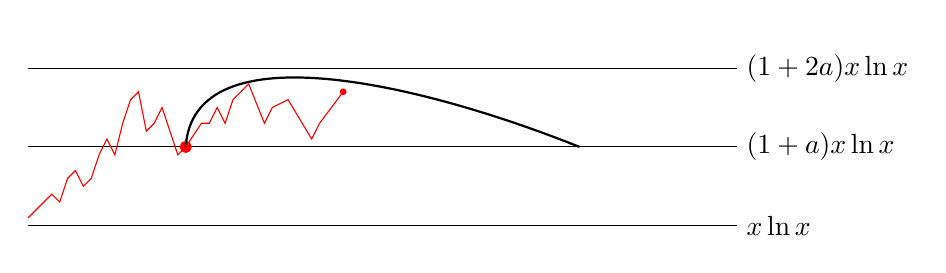
\begin{tikzpicture}
    \draw (-2,0)--(7,0) node[anchor=west] {$x\ln{x}$};
    \draw (-2,1)--(7,1) node[anchor=west] {$(1+a)x\ln{x}$};
    \draw (-2,2)--(7,2) node[anchor=west] {$(1+2a)x\ln{x}$};
    \draw[red] (-2,0.1)--(-1.8,0.3)--(-1.7,0.4)--(-1.6,0.3)--(-1.5,0.6)--(-1.4,0.7)--(-1.3,0.5)--(-1.2,0.6)--(-1.1,0.9)--(-1,1.1)--(-0.9,0.9)--(-0.8,1.3)--(-0.7,1.6)--(-0.6,1.7)--(-0.5,1.2)--(-0.4,1.3)--(-0.3,1.5)--(-0.2,1.2)--(-0.1,0.9)--(0,1);
    \filldraw[red] (0,1) circle (2pt);
    \draw[thick] (0,1) ..controls (0.1, 2.5) and (3,1.8).. (5,1);
    \draw[red] (0,1)--(0.2,1.3)--(0.3,1.3)--(0.4,1.5)--(0.5,1.3)--(0.6,1.6)--(0.8,1.8)--(1,1.3)--(1.1,1.5)--(1.3,1.6)--(1.6,1.1)--(1.7,1.3)--(2,1.7);
    \filldraw[red] (2,1.7) circle (1pt);
\end{tikzpicture}

\end{document}